\documentclass[tikz,border=10pt]{standalone}
\usepackage{tikz}
\usetikzlibrary{shapes.geometric,arrows.meta,positioning,calc,backgrounds,shadows,decorations.pathmorphing}
\usepackage[T1]{fontenc}
\usepackage{amssymb}
\usepackage{helvet}\renewcommand{\familydefault}{\sfdefault}
\usepackage[tracking=true]{microtype}

\definecolor{bandA}{HTML}{BBD4F5}
\definecolor{bandB}{HTML}{CDBCEC}
\definecolor{bandC}{HTML}{B9E3C6}
\definecolor{secA}{HTML}{3E6FB4}
\definecolor{secB}{HTML}{6E51A8}
\definecolor{secC}{HTML}{3F8A5E}
\definecolor{cardEdge}{HTML}{51607A}
\definecolor{boxblue}{HTML}{BFD8F7}
\definecolor{boxpurple}{HTML}{D6C8F0}
\definecolor{boxgreen}{HTML}{BFE5CC}
\definecolor{chipadv}{HTML}{F6C7C4}
\definecolor{chipnat}{HTML}{FADFB8}
\definecolor{chipben}{HTML}{CBE9BC}
\definecolor{dbcol}{HTML}{F3E1A8}
\definecolor{dbtop}{HTML}{EAD285}
\definecolor{ink}{HTML}{273244}
\definecolor{sub}{HTML}{5B6779}
\definecolor{arrowc}{HTML}{7A8698}
\definecolor{hi}{RGB}{212,241,212}
\definecolor{lo}{RGB}{250,214,214}
\definecolor{trajgood}{HTML}{35B26A}
\definecolor{trajbad}{HTML}{E4574B}


\tikzset{
  every node/.style={font=\small, text=ink},
  card/.style={draw=cardEdge!45, rounded corners=2.4mm, fill=white,
               inner sep=2.6mm, line width=0.6pt,
               drop shadow={opacity=0.12, shadow xshift=0.35mm, shadow yshift=-0.55mm,
                            fill=black}},
  model/.style={card, fill=boxblue, minimum width=17mm, minimum height=10mm,
                font=\small\bfseries},
  modelp/.style={model, fill=boxpurple},
  modelg/.style={model, fill=boxgreen},
  chip/.style={draw=cardEdge!35, rounded corners=1.7mm, inner xsep=2.2mm,
               inner ysep=1.5mm, font=\footnotesize, line width=0.5pt,
               drop shadow={opacity=0.10, shadow xshift=0.3mm, shadow yshift=-0.45mm,
                            fill=black}},
  db/.style={cylinder, shape border rotate=90, draw=cardEdge!50, fill=dbcol,
             cylinder uses custom fill, cylinder body fill=dbcol, cylinder end fill=dbtop,
             aspect=0.16, minimum width=14.5mm, minimum height=12.5mm,
             inner sep=1.1mm, line width=0.6pt, font=\footnotesize\bfseries,
             drop shadow={opacity=0.12, shadow xshift=0.35mm, shadow yshift=-0.55mm,
                          fill=black}},
  arr/.style={-{Stealth[length=2.7mm, width=2.2mm]}, line width=0.8pt,
              draw=arrowc, rounded corners=2mm},
  lab/.style={font=\footnotesize, text=sub, inner sep=1pt},
}

\begin{document}
\begin{tikzpicture}

% ================= EVIDENCE GATHERING (top) =================
\node[card, align=center, inner sep=2.0mm] (task) at (0,0) {%
  \begin{tabular}{@{}c@{}}
  {\footnotesize\bfseries task}\\[0.4mm]
  {\tiny\color{sub}scene}\\[0.3mm]
  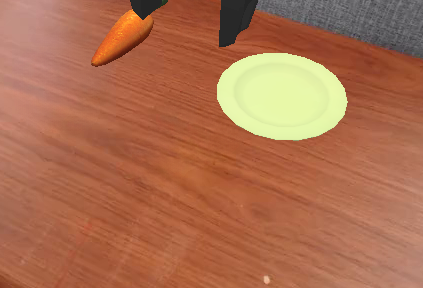
\includegraphics[width=26mm]{frames/method_frame.png}\\[0.4mm]
  {\tiny\color{sub}instruction}\\[0.2mm]
  {\footnotesize``move the carrot to the plate''}
  \end{tabular}};

\node[model] (vlm1) at (3.45,0) {VLM};
\draw[arr] (task) -- (vlm1);

% two rephrase mini-cards with rollout overlays
\node[card, inner sep=1.2mm, align=center] (mcA) at (6.55,1.18) {%
  \begin{tabular}{@{}c@{}}
  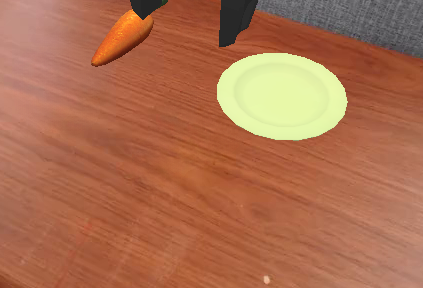
\includegraphics[width=20mm]{frames/method_frame.png}\\[0.3mm]
  {\tiny``move the carrot to the dish''}
  \end{tabular}};
\node[card, inner sep=1.2mm, align=center] (mcB) at (6.55,-1.18) {%
  \begin{tabular}{@{}c@{}}
  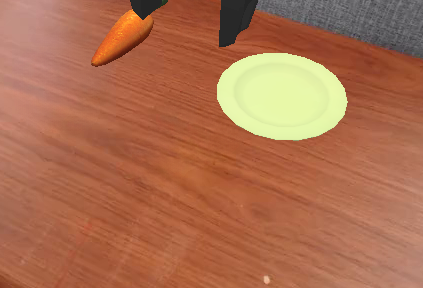
\includegraphics[width=20mm]{frames/method_frame.png}\\[0.3mm]
  {\tiny``place the carrot on the yellow plate''}
  \end{tabular}};

\begin{scope}[decoration={random steps, segment length=0.9mm, amplitude=0.22mm},
              trj/.style={line width=0.55pt, line cap=round, decorate,
                          -{Stealth[length=1.1mm, width=1.0mm]}}]
% card A: 1 green, 3 red
\begin{scope}[shift={($(mcA.center)+(0,0.30)$)}]
\draw[trj, trajgood] (0.05,0.14) .. controls (-0.10,-0.04) and (-0.12,-0.22) .. (0.15,-0.30);
\draw[trj, trajbad]  (0.05,0.14) .. controls (0.28,0.18)  and (0.50,0.04)  .. (0.70,0.10);
\draw[trj, trajbad]  (0.05,0.14) .. controls (-0.28,0.10) and (-0.55,-0.02) .. (-0.70,-0.12);
\draw[trj, trajbad]  (0.05,0.14) .. controls (0.12,-0.14) and (0.38,-0.34) .. (0.55,-0.44);
\end{scope}
% card B: 3 green, 1 red
\begin{scope}[shift={($(mcB.center)+(0,0.30)$)}]
\draw[trj, trajgood] (0.05,0.14) .. controls (-0.10,-0.04) and (-0.12,-0.22) .. (0.15,-0.30);
\draw[trj, trajgood] (0.05,0.14) .. controls (0.02,-0.08)  and (0.06,-0.20)  .. (0.20,-0.26);
\draw[trj, trajgood] (0.05,0.14) .. controls (-0.18,0.02)  and (-0.22,-0.32) .. (0.22,-0.36);
\draw[trj, trajbad]  (0.05,0.14) .. controls (0.28,0.16)  and (0.48,0.06)  .. (0.66,0.12);
\end{scope}
\end{scope}

\draw[arr] (vlm1) -- node[lab, above=0.8mm, align=center, pos=0.35]{rephrase\\[-0.2mm]\& score} ($(mcA.west)+(-0.05,-0.2)$);
\draw[arr] (vlm1) -- ($(mcB.west)+(-0.05,0.2)$);

% evidence panel: three minimal pairs
\node[card, align=left, inner sep=1.8mm] (evidence) at (10.9,0) {%
  \begin{tabular}{@{}l@{\hspace{2.5mm}}r@{}}
  \multicolumn{2}{c}{\footnotesize\bfseries evidence}\\[0.8mm]
  {\tiny``\colorbox{lo}{\strut move} the carrot\,\ldots''} & {\tiny 25\%}\\[0.2mm]
  {\tiny``\colorbox{hi}{\strut put} the carrot\,\ldots''} & {\tiny 50\%}\\[1.1mm]
  {\tiny``\ldots\,on the \colorbox{lo}{\strut plate}''} & {\tiny 15\%}\\[0.2mm]
  {\tiny``\ldots\,on the \colorbox{hi}{\strut yellow plate}''} & {\tiny 30\%}\\[1.1mm]
  {\tiny``\ldots\,\colorbox{lo}{\strut dish}''} & {\tiny 10\%}\\[0.2mm]
  {\tiny``\ldots\,\colorbox{hi}{\strut plate}''} & {\tiny 60\%}
  \end{tabular}};
\draw[arr] ($(mcA.east)+(0.05,-0.2)$) -- ($(evidence.west)+(-0.05,0.3)$);
\draw[arr] ($(mcB.east)+(0.05,0.2)$) -- ($(evidence.west)+(-0.05,-0.3)$);

% ================= RULE DISTILLATION (right rail) =================
\node[modelp] (llm) at (10.9,-2.9) {LLM};
\draw[arr] (evidence) -- (llm);
\node[card, align=left, inner sep=1.8mm] (rules) at (10.9,-5.0) {%
  \begin{tabular}{@{}l@{}}
  \multicolumn{1}{c}{\footnotesize\bfseries rules}\\[0.6mm]
  {\tiny 1. prefer `put' over `move', `place', \ldots}\\[0.2mm]
  {\tiny 2. prefer common nouns: keep `plate',}\\[-0.2mm]
  {\tiny \phantom{2. }not `dish'}\\[0.1mm]
  \multicolumn{1}{c}{{\scriptsize$\vdots$}}
  \end{tabular}};
\draw[arr] (llm) -- node[lab, right=1.2mm]{distill} (rules);

% ================= RULE APPLICATION (bottom) =================
\node[card, align=center, inner sep=1.6mm] (task2) at (5.1,-4.02) {%
  \begin{tabular}{@{}c@{}}
  {\footnotesize\bfseries task}\\[0.3mm]
  {\tiny\color{sub}scene}\\[0.2mm]
  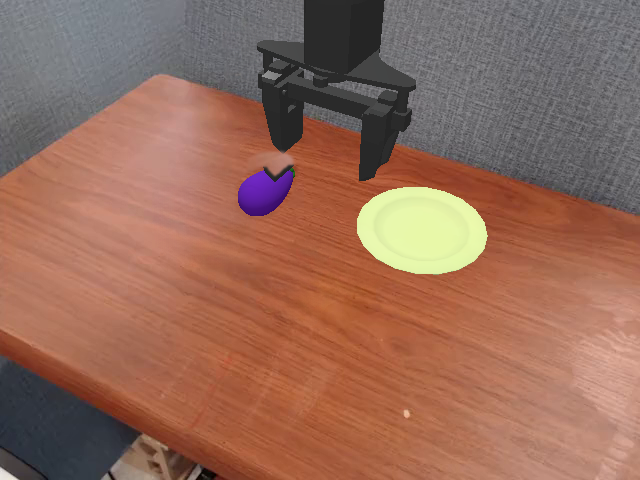
\includegraphics[width=17mm]{frames/eggplant_plate_composite.png}\\[0.3mm]
  {\tiny\color{sub}instruction}\\[0.1mm]
  {\scriptsize``Can you move the eggplant to the dish?''}
  \end{tabular}};

\node[modelg] (vlm2) at (7.9,-6.08) {VLM};
\node[card, align=center] (reph) at (3.9,-6.08) {%
  {\scriptsize``put the eggplant on the plate''}};
\node[model] (vla2) at (0.6,-6.08) {VLA};
\draw[arr] (rules) -- (vlm2);
\draw[arr] (task2) -- (vlm2);
\draw[arr] (vlm2) -- node[lab, below=0.7mm]{rephrase} (reph);
\draw[arr] (reph) -- (vla2);

% ================= bands =================
\begin{scope}[on background layer]
  \fill[bandA, fill opacity=0.38, rounded corners=4mm]
      (-1.95,1.95) rectangle (12.95,-2.15);
  \fill[bandB, fill opacity=0.38, rounded corners=4mm]
      (9.55,1.95) rectangle (12.95,-6.6);
  \fill[bandC, fill opacity=0.38, rounded corners=4mm]
      (-1.95,-3.05) rectangle (9.1,-6.6);
\end{scope}

% ================= section labels =================
\node[anchor=south west, font=\normalsize\bfseries, text=secA]
  at (2.05,2.05) {\textls[130]{EVIDENCE GATHERING}};
\node[anchor=center, rotate=-90, font=\normalsize\bfseries, text=secB]
  at (13.35,-2.3) {\textls[130]{RULE DISTILLATION}};
\node[anchor=south west, font=\normalsize\bfseries, text=secC]
  at (-1.9,-2.98) {\textls[130]{RULE APPLICATION}};

\end{tikzpicture}
\end{document}
